\lecture{4}{25.09.2020}{Método da Função Descritiva}

Precisamos de um método prático para detectar e analisar \emph{ciclos limites}. Particularmente útil para sistemas lineares com \emph{não-linearidades estáticas}, tais como: saturação, relê, quantizador, histerese e zona morta.

Formulamos o problema como
\begin{figure}[H]
    \centering
    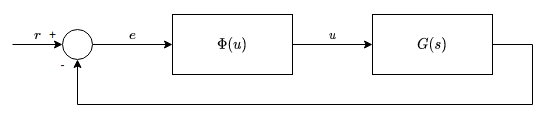
\includegraphics[width=0.6\textwidth]{figures/plant_with_nonlinear_static.png}
\end{figure}
onde $\Phi$ é uma função não linear estática. Queremos, então, aproximar a não-linearidade por um ganho para uma entrada $e(t) = A\sin\omega t$.

Por Fourier, sabemos que \[
    \Phi(u(t)) = C_0 + \sum_{n=1}^{\infty} A_n\cos\left( n\omega t \right) + B_n\sin\left( n\omega t \right) 
\] com coeficientes determinados por
\begin{align*}
    C_0 = \frac{1}{2\pi}\int_0^{2\pi}\Phi\left( u(\tau) \right) d\tau \\
    A_k = \frac{1}{\pi}\int_0^{2\pi}\Phi\left( u(\tau) \right) \cos k\tau d\tau \\
    A_k = \frac{1}{\pi}\int_0^{2\pi}\Phi\left( u(\tau) \right) \sin k\tau d\tau \\
.\end{align*}

Para uma boa aproximação, podemos utilizar somente os primeiros termos da séries de Fourier, portanto \[
\Phi\left( u(t) \right) \cong C_0 + A_1\cos\omega t + B_1\sin\omega t
\] e, se estamos lidando com uma entrada com média nula, temos $C_0 = 0$. 

Algumas propriedades dessa aproximação:
\begin{itemize}
    \item A amplitude do sinal pode ser calculada como $\sqrt{A_1^2 + B_1^2}$;
    \item Funções ímpares, simétricas tais que $\Phi(u) = -\Phi(-u)$, possuem $A_1=0$;
    \item Funções pares, simétricas tais que $\Phi(u) = \Phi(-u)$, possuem $B_1=0$.
\end{itemize}

Temos, então, a relação entrada-saída dessa função \[
    \frac{u(t)}{e(t)} = \frac{C_0 + A_1\cos\omega t + B_1\sin\omega t}{A\sin\omega t} = \frac{\sqrt{A_1^2 + B_1^2} \sin\left( \omega t + \varphi \right) }{A\sin\omega t}
\], onde $\varphi = tg^{-1}\left( \frac{A_1}{B_1} \right) $. Portanto, temos um ganho equivalente aproximado \[
N(A) = \frac{\sqrt{A_1^2 + B_1^2}}{A} \angle \varphi
\].

Assim, podemos modelar o sistema utilizando o ganho equivalente da não-linearidade. Define-se o sistema em malha aberta desconsiderando a não-linearidade \[
    P(s) = C(s)G(s)
\]. Agora, a estabilidade do sistema é determinada pela equação característica \[
1 + N(A)P(s) = 0
\] e podemos utilizar, por exemplo, Nyquist através de \[
P(j\omega) = \frac{-1}{N(A)}
\]. A ideia é encontrar o ciclo limite no ponto crítico do sistema. Assim, encontramos o ganho e fase do ciclo limite através de \[
\begin{cases}
    \Im\left( P(j\omega_c \right) = 0 \\
    \Re\left( P(j\omega_c \right) = \frac{-1}{N(A_c)}
\end{cases}
\].

A condição de estabilidade do ciclo limite é de que \[
    \frac{d N(A)}{dA}\Bigr|_{A=A_c} \frac{d \Im\left( P(j\omega) \right) }{d\omega}\Bigr|_{\omega=\omega_c} < 0
\].

